% ============================================================
% paper/figures.tex
% Figures: Structural Illustrations (Executable-Closed)
% ============================================================

\section*{Figures and Visual Material}

\subsection*{Role and Interpretation of Figures}

The figures included in this document serve a strictly illustrative and
structural purpose.
They visualize consequences of the executable specification
\texttt{ETS.K\_EA.v1.1} under selected instantiations and parameter
choices.

Figures do not introduce new theoretical content.
They do not define primitives, parameters, thresholds, admissible
transitions, or phase logic.
All formal meaning is defined exclusively by the Executable Theory
Specification and the main text of this whitepaper.

The figures are provided solely to support inspection of:
\begin{itemize}
  \item admissible versus non-admissible regions of state space,
  \item qualitative behavior of threshold components,
  \item interaction between continuity $k_{\mathrm{EA}}$, cycles, and
        termination conditions,
  \item phase classification implied by structural constraints.
\end{itemize}

\subsection*{Non-Empirical Status}

All figures are generated from synthetic instantiations of the
executable specification.
They are not empirical measurements, benchmarks, validation data, or
case evidence.

They do not support predictive claims, comparative assessment, or
generalization across enterprises.

Their role is analogous to consistency diagrams in formal systems: they
illustrate structural behavior implied by the specification without
asserting factual truth about real-world enterprises.

\subsection*{Included Figures}

\begin{figure}[H]
\centering
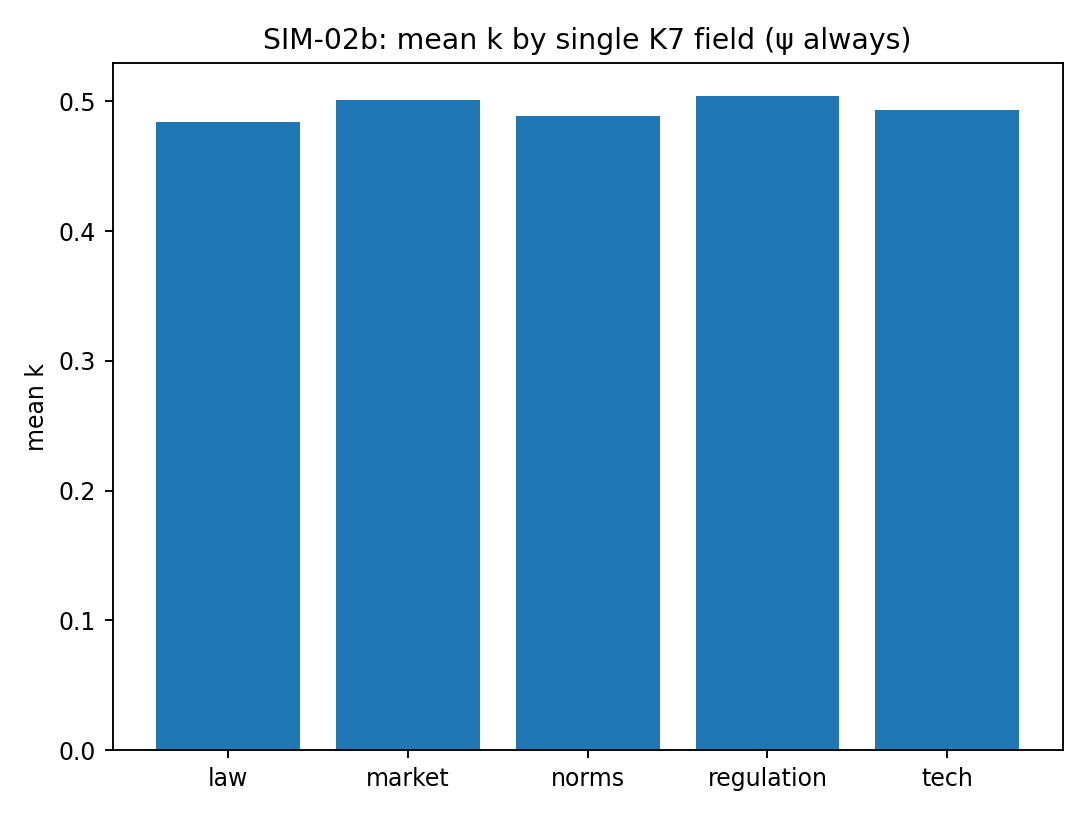
\includegraphics[width=0.9\linewidth]{figures/sim02b_mean_k_by_field.png}
\caption{Illustrative aggregation of continuity contributions under
different external field instantiations.
The figure visualizes structural sensitivity of $k_{\mathrm{EA}}$ to
field-level constraints.
No empirical interpretation is implied.}
\end{figure}

\begin{figure}[H]
\centering
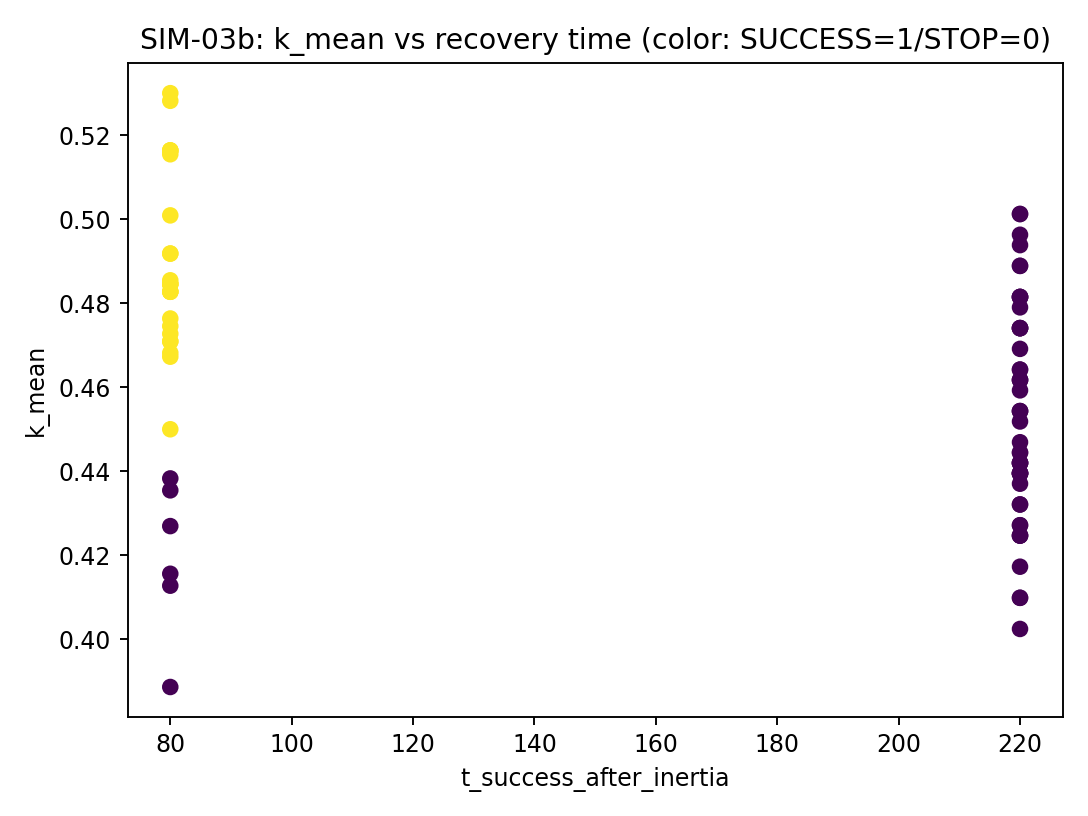
\includegraphics[width=0.9\linewidth]{figures/sim03b_k_vs_tsuccess.png}
\caption{Relationship between continuity and median success time under
synthetic instantiation.
The figure illustrates internal consistency of phase logic rather than
performance behavior.}
\end{figure}

\begin{figure}[H]
\centering
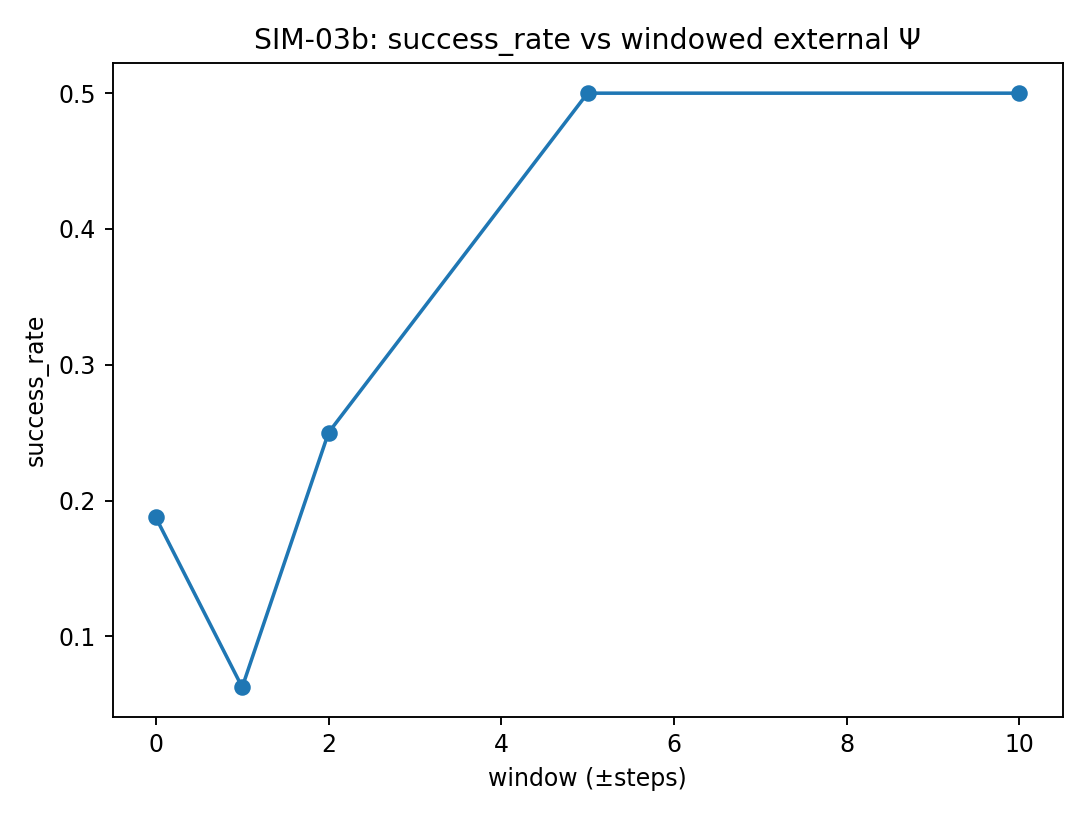
\includegraphics[width=0.9\linewidth]{figures/sim03b_success_rate_vs_window.png}
\caption{Phase outcome frequencies under varying observation windows.
The visualization reflects structural dependence on observability
constraints, not empirical success rates.}
\end{figure}

\begin{figure}[H]
\centering
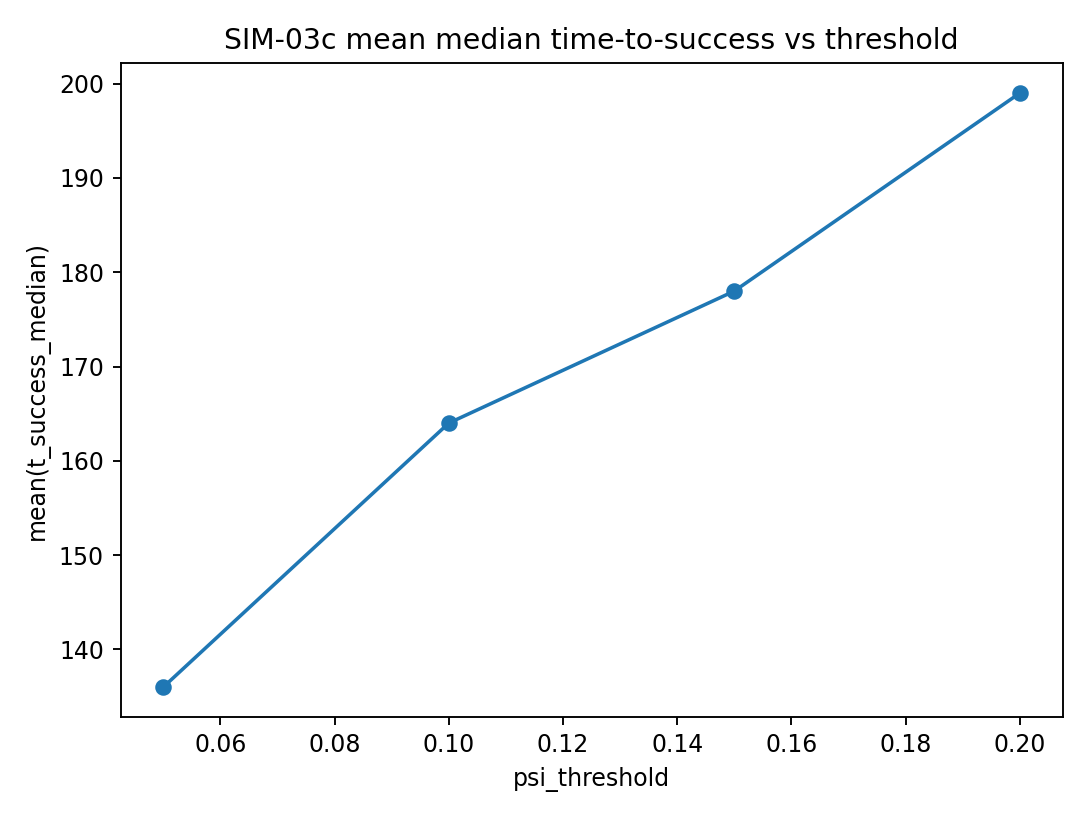
\includegraphics[width=0.9\linewidth]{figures/sim03c_tsuccess_median_vs_threshold.png}
\caption{Median transition times as a function of threshold
instantiation.
Shown values illustrate admissibility boundaries implied by the ETS.}
\end{figure}

\subsection*{Heatmap Series}

The following heatmaps visualize admissible and non-admissible regions
of the enterprise state space under varying window and threshold
parameters.
They illustrate structural phase boundaries and STOP regions implied by
the executable specification.

\begin{figure}[H]
\centering
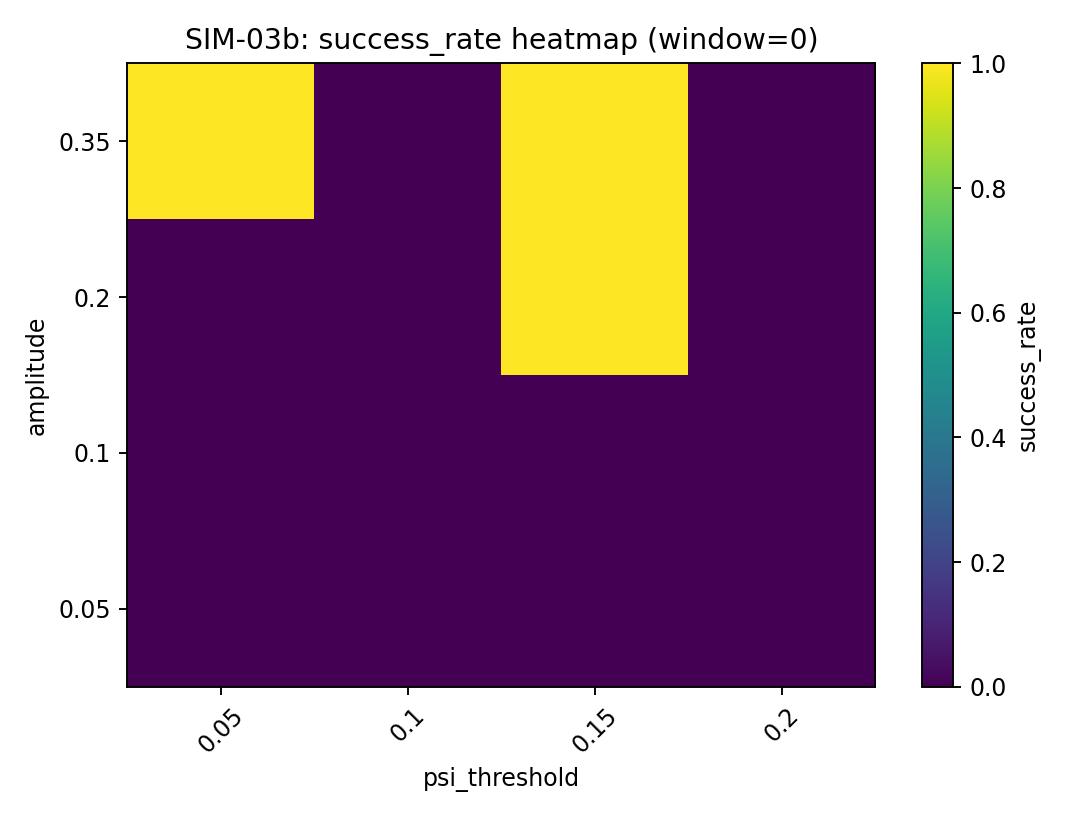
\includegraphics[width=0.9\linewidth]{figures/sim03b_heatmap_window_0.png}
\caption{Admissibility heatmap for window parameter $w = 0$.}
\end{figure}

\begin{figure}[H]
\centering
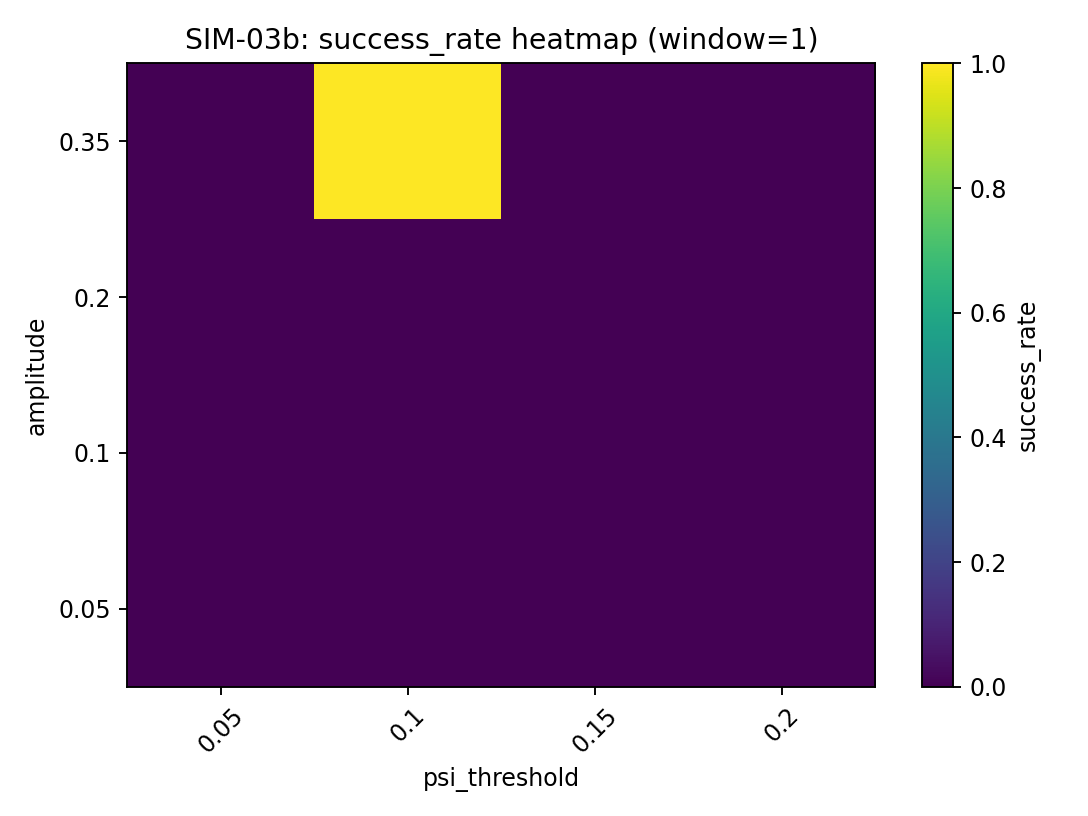
\includegraphics[width=0.9\linewidth]{figures/sim03b_heatmap_window_1.png}
\caption{Admissibility heatmap for window parameter $w = 1$.}
\end{figure}

\begin{figure}[H]
\centering
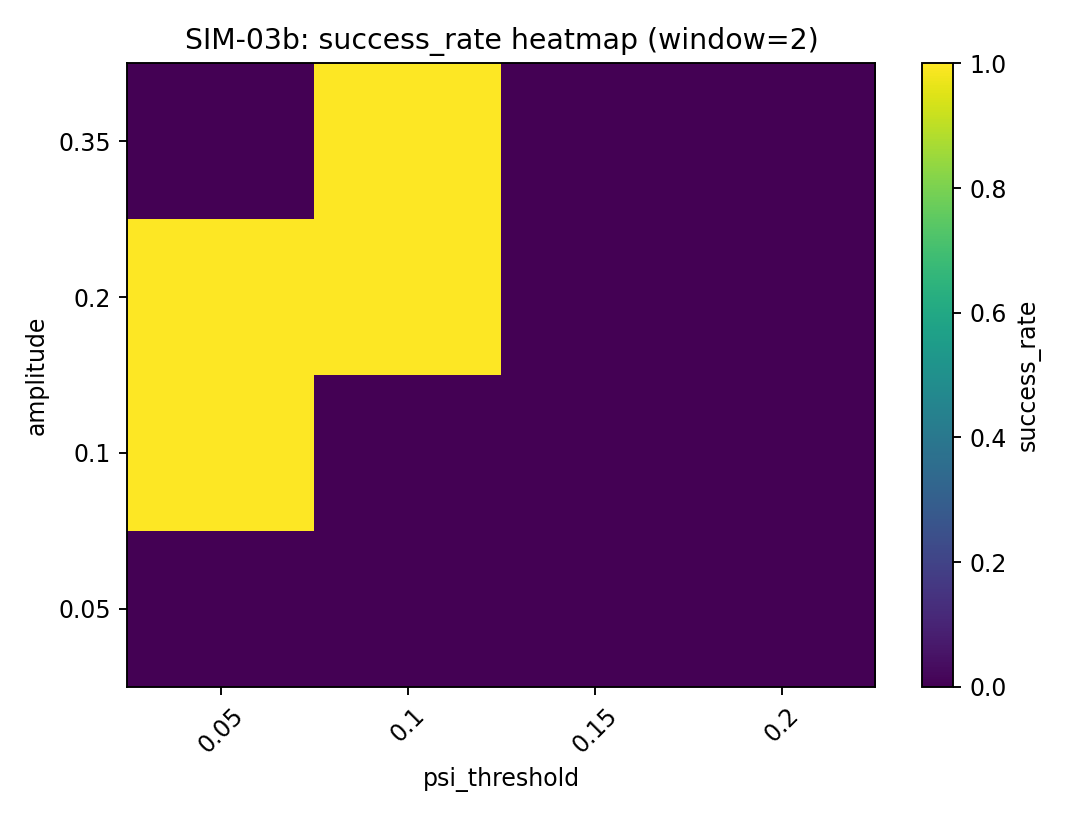
\includegraphics[width=0.9\linewidth]{figures/sim03b_heatmap_window_2.png}
\caption{Admissibility heatmap for window parameter $w = 2$.}
\end{figure}

\begin{figure}[H]
\centering
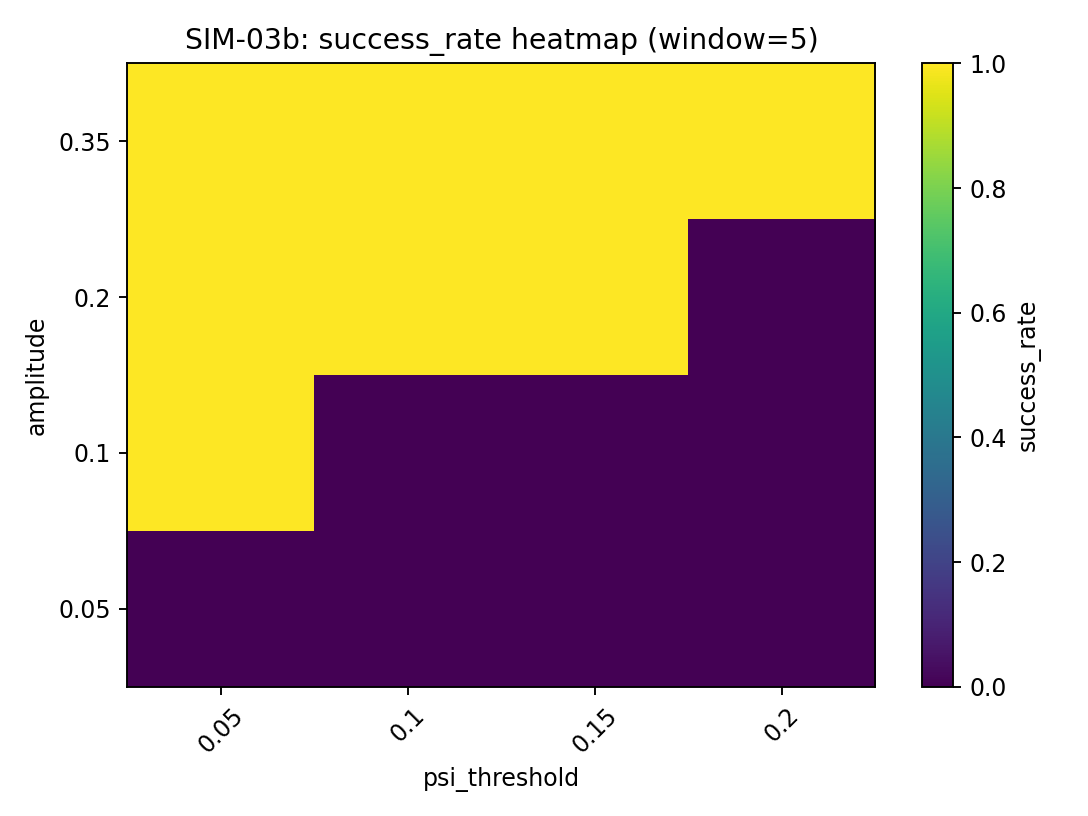
\includegraphics[width=0.9\linewidth]{figures/sim03b_heatmap_window_5.png}
\caption{Admissibility heatmap for window parameter $w = 5$.}
\end{figure}

\begin{figure}[H]
\centering
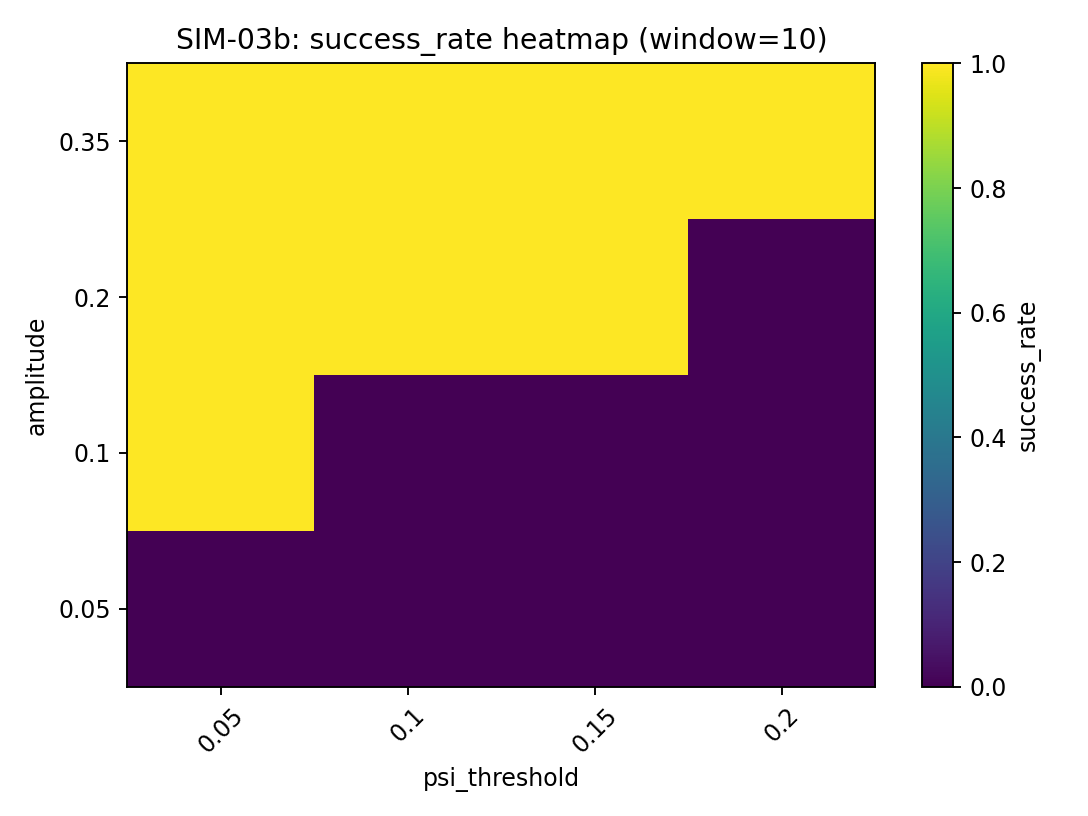
\includegraphics[width=0.9\linewidth]{figures/sim03b_heatmap_window_10.png}
\caption{Admissibility heatmap for window parameter $w = 10$.}
\end{figure}

\subsection*{Interpretation Boundary}

Figures carry no independent diagnostic authority.

No figure may be used to bypass STOP conditions, invariants, compatibility
constraints, or phase precedence rules.
If a visual pattern appears to contradict a formal result, the formal
specification takes precedence.

%%%End of Document%%%
